% Hetedik előadás

\chapter{ARM processzorok}

Az ARM az Intel és az AMD mellett a harmadik nagy szereplő, a mobil világban egyeduralkodó.

\section{Terminológia}
Az ARM nem processzorgyártó cég, hanem CPU-kat, GPU-kat, NPU-kat és egyebeket fejlesztenek és a szellemi tulajdont értékesítik.
Ezzel szemben az Intel, AMD, Qualcomm stb. komplett processzorokat fejlesztenek és forgalmaznak, részben az ARM szellemi tulajdona alapján.
Ezért az ARM-re CPU - és nem processzor - fejlesztőként hivatkozunk.

\section{Áttekintés}
Az ARM egy brit félvezető fejlesztő cég (1983-ban alapították, Acorn RISC Machine, de 1990-től az Apple és a VLSI-vel közös projekttel Advanced RISC Machines), amit 2016-ban megvett egy japán bank, a Softbank.
2021-ben az Nvidia bejelntette, hogy megveszi az ARM-et, de ez még folyamatban van.
A cég alapvetően tervezéssel foglalkozik, kis áramfogyasztású processzor komponenseket és ezekhez kapcsolódó tervezési eszközöket fejleszt.
Ezek szellemi termékek, a bevételük ezeknek a licenszeléséből származik.

\subsection{Üzleti modell}
Az ARM a technológiát licenszeli a félvezető gyártó partnereinek, akik ezért licenszdíjat fizetnek.
A félvezető gyártó a legyártott processzorokat eladja az OEM gyártóknak (közben royalty-t fizetnek az ARM-nek), az OEM gyártók pedig végfelhasználói termékeket értékesítenek.
Az ARM figyelembe veszi a partnerek visszajelzéseit.
\begin{figure}[H]
    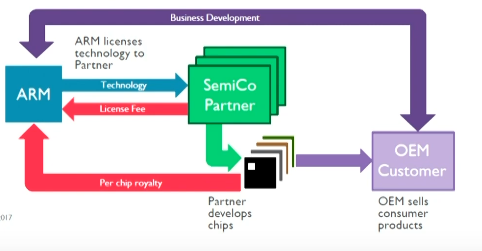
\includegraphics[width=0.7\textwidth]{armbm}
    \centering
    \caption{Az ARM üzleti modellje}
    \label{fig:armbm}
\end{figure}

\subsection{Licenszelés}
Az ARM két licenszet forgalmaz:
\begin{itemize}
    \item Cortex licensz: az ARM egy komplett mikroarchitektúrát értékesít, konfigurálható opciókkal
    \item Architektúra licensz: az ARM csak az ISA-t adja át a vevőnek, a vevő dolga megtervezni a saját mikroarchitektúráját (pl. Apple és Samsung)
\end{itemize}

\subsection{Az ARM dominanciájának okai}
Az ARM az x86-al szemben egy RISC architektúra, a RISC pedig Load/Store architektúra, tehát az operandusokat a regiszterekből olvassa be.
Az x86 viszont CISC és megenged operandus olvasást közvetlenül a memóriából.
Következmények:
\begin{itemize}
    \item a CISC utasítások nagyon hosszúak lehetnek a memória címzése miatt (base reg, offset, stb.)
    \item a RISC-eknél az utasításoknál elég a regisztereken címezni, a Load/Store-nál pedig a memóriát
    \item a CISC-ek utasításhossza változó, a RISC fix (általában 32 bit)
    \item a CISC-ek több áramot fogyasztanak, mivel az utasítás lehívás és a dekódolás komplexebb
\end{itemize}
A mobil világban nagyon fontos az alacsony fogyasztás, ezért a RISC alapú ARM architektúrák előnye.
Az ARM processzorok további fejlődésben vannak, újabban a szervereknél is kezdenek teret nyerni.
2020-ban, mikor az ARM-et megvette az Nvidia, az Nvidia CEO-ja kijelentette, hogy a desktopoknál is a legfontosabb architektúra az ARM lesz a jövőben.

\section{Az ARM ISA fejlődése}
 Az ARM (RISC) architektúra kezdetben kevés utasítást tartalmazott, de később az utasítások száma meghaladta az x86-ost is.
 Napjainkig 9 különböző ARM ISA verziót hoztak ki.
 Az első két verzióban még csak 26 bites címteret használt.
 Az ARMv3 volt az első olyan ISA verzió, ami már 32 bites címteret használt, ez tekinthető az ARM kiindulópontjának.
 Az ARM ISA jellemzői (korai változatok):
 \begin{itemize}
     \item 32 bites RISC architektúra
     \item 32 bites fixpontos vagy logikai adatokkal képes dolgozni
     \item 16 regisztert tartalmaz (13 általános + 3 dedikált)
 \end{itemize}
 A fejlődés négy fő irányban történt:
 \begin{itemize}
     \item számítási képességek növelése
     \item programkód méretének csökkentése
     \item bytekód végrehajtási sebesség növelése
     \item biztonság fokozása
 \end{itemize}
 A korai ARM rendszerek egyszerű, beágyazott alkalmazásokhoz készültek, ahol fontos volt a kód mérete és a bytekód végrehajtás sebessége is kritikus.
 A 2000-es években az ARM utat talált az alkalmazói processzorokba (mobilok), ahol sokkal általánosabb feladatokat kellett végrehajtania.
 Megjelent tehát a grafika és így a lebegőpontos számításokra való igény, megjelentek a SIMD utasítások is a számítási teljesítmény növelése érdekében.
 Fontossá vált a biztonság is.
 A v7-től kezdve a korábban fontosnak tartott szempontok értelmüket vesztették.

 \section{Számítási képességek fejlődése}
 Az ARMv3 egy egyszerű, alap architektúra, amit a fejlődés során kiterjesztettek.
 Egy utasításkészlet kiterjesztéséhez két dologra van szükség: egy regiszterkészlet definiálására és a regisztereken végrehajtható utasítások meghatározására.
 Az ARN fejlesztése három fő logikai lépésből állt:
 \begin{itemize}
     \item a műveletek kiterjesztése fixpontos SIMD utasításokkal (2002, ARMv6)
     \item másodlagos regiszterkészlet bevezetése skalár lebegőpontos, SIMD lebegőpontos és FX/FP lebegőpontos műveletekhez (2000, ARMv5)
     \item SVE regiszterkészlet (nagyon széles, 2KB) bevezetése, erre alapozva utasításkészlet kiegészítése (2016, ARMv8.2)
 \end{itemize}

 \subsection{Fixpontos SIMD kiterjesztés}
 Ezzel 32 bit szélesen lehetett végrehajtani 8 vagy 16 bites műveleteket (\ref{fig:fxsimd}).
 \begin{figure}[H]
    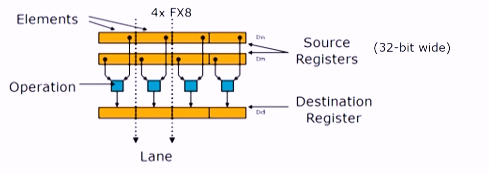
\includegraphics[width=0.7\textwidth]{fxsimd}
    \centering
    \caption{Fixpontos SIMD utasítások végrehajtása}
    \label{fig:fxsimd}
\end{figure}
Az ezzel elért teljesítmény növekedés csekély volt, ezért később kiterjesztették a NEON bővítménnyel.

Az ARMv8 ISA-jának két végrehajtási módja volt: 32 és 64 bites.
Az utóbbihoz kiterjesztették a regiszterkészletet, a 32 bites működés a kompatibilitást szolgálta.

\subsection{Lebegőpontos műveletvégzés}
A NEON kiterjesztés a multimédiás alkalmazások gyorsítását szolgálta.
Lehetővé tette, hogy 64 vagy 128 bites hosszú adatokon történjen a műveletvégzés.

\subsection{SVE regiszterkészletre alapuló SIMD kiterjesztések}
Az SVE-t (Scalable Vector Extension) 2016-ban mutatták be, az ARMv8.2 alapú ISA-ban.
Csak a 64 bites verzióban volt aktív.
Alapvető célja a HPC (High Performance Computing), tehát a tudományos jellegű, képfeldolgozó és média alkalmazások támogatása.
FX és FP műveleteket is támogat.
A regiszterkészlet nem volt rögzítve, hanem 128 bittől egészen 2 Kb hosszú regiszterek használhatók voltak, tehát többféle fixpontos és lebegőpontos adattípust is támogatott.
Ezeket hívták Z regisztereknek.

Legfontosabb jellemzője, hogy a programozásban nem kell figyelembe venni a hardveres regiszterek hosszát.
Így a programozóknak könnyebb kódot írnia, mivel eltérő végrehajtóegység méretű processzorokra ugyanazt a kódot tudja használni.
A megírt binárisok hordozhatóbbak és automatikus vektorizáció lehetséges a compilerekben.

A megvalósításhoz predikátum regisztereket vezettek be, amiket maszkokként használtak.
Ez megmutatja, hogy az adat melyik része aktív és melyik nem.
16 predikátum regiszter áll rendelkezésre.
A predikátum regisztereket a programkódban be kell állítani.

\subsection{SVE 2}
Az előző részben leírt SVE-t szinte nem használták.
Később bemutatták a továbbfejlesztett változatát, az SVE2-t (ARMv9, 2021).
A cél a HPC helyett egy széleskörű alkalmazás palettát támogatni és a NEON-t kiváltani.
\begin{figure}[H]
    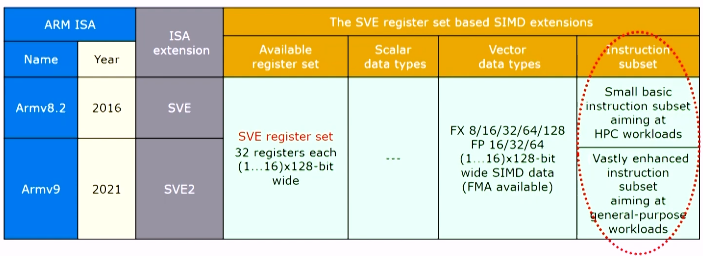
\includegraphics[width=0.8\textwidth]{sve}
    \centering
    \caption{Az SVE és SVE2 összehasonlítása}
    \label{fig:sve}
\end{figure}
Az SVE-t csak a Fujitsu A64FX processzora implementálta.
Ennek oka, hogy az eredeti SVE nagyrészt HPC feladatokra volt kitalálva, de a mobilok nem futtatnak ilyen alkalmazásokat.
Ezzel szemben az SVE2 elsősorban a szervereket célozza meg, ahol gyakoriak az ilyen feladatok.

\section{Az ARM CPU-k áttekintése}
Az ARM CPU-k csoportosítása:
\begin{itemize}
    \item Korai ARM CPU-k
    \begin{itemize}
        \item ARMv1 és v2 (1985-1990): 26 bites címbuszú rendszerek, nem tárgyaljuk őket. Pl.: ARM1-ARM3
        \item ARMv3-v6 (1991-2004): 32 bites rendszerek. Pl.: ARM6xx-ARM11xx
    \end{itemize}
    \item ARM Cortex CPU-k (ARMv7-v9): 2004-től, ma is ezek az uralkodók. 8.0-tól 64 bites
    \item ARM Neoverse CPU-k (ARMv9): 2021-től, szerverekhez készültek, teljesen új család
\end{itemize}

\subsection{Cortex CPU-k}
A Cortex CPU-k a jelenlegi mobil világ alapját alkotják.
2004-ben vezették be, elsőként a Cortex-M3 beágyazott processzorban.

\subsection{Cortex profilok}
A Cortex családot 3 különböző profilra osztották, felhasználás szerint:
\begin{itemize}
    \item Cortex-A: alkalmazások
    \item Cortex-R: kritikus, valós idejű rendszerek
    \item Cortex-M: mikrokontroller, nem annyira kritikus rendszerek
\end{itemize}

\subsubsection{Cortex-A profil}
Két utasításkészletet támogat: az A32-t és a T32-t.
A T32 egy 16 bites utasításokat tartalmazó részhalmaza az A32-nek.
Az ARMv8-A verzióval megjelent a 64 bites kiterjesztés, a korábbi 32 bites alkalmazásokkal kompatibilis módon.
A 32 bites alkalmazásokat AArch32 végrehajtási módban, A32 utasításkészlettel futtatja, a 64 biteseket pedig AArch 64 módban, A64 utasításkészlettel.
Ezzel együtt az AArch64 módban megszüntették a Thumb 16 bites utasításkészlet támogatását.
Az ARMv9-el a 32 bites utasításokat sem támogatták tovább.

\subsubsection{Cortex-R profil}
Beágyazott rendszerekhez készült, szintén az A32 és T32 utasításkészleteket támogatja.

\subsubsection{Cortex-M profil}
Mélyen beágyazott rendszerekhez, mikrokontrollerekhez készült (pl. autóipar).
Ez csak a T32 16 bites utasításokat támogatja.

\subsubsection{SecurCore profil}
2007-ben a családot kiegészítették a SecurCore profillal, smart card és egyéb biztonsági alkalmazásokra kifejlesztve.

\subsection{A Cortex-A profilú CPU-k fejlődése}
2004-ben jelentek meg az első Cortex-A CPU-k, 2011-től támogatták a big.LITTLE felépítést (ARMv7-A ISA).
Ezt követték az ARMv8-A-t megvalósító, 64 bites CPU-k (2012-ben jelentették be).
A következő generáció (ARMv8.2-A, 2017) már támogatta DynamIQ magcsoportokat, ami a korábbi big.LITTLE magcsoportokat váltotta.
2021-ben megjelent az ARMv9-A, ahol jelentősen továbbfejlesztették a DynamIQ-t.

\subsubsection{Az ARMv7-8 CPU-k fejlődése}
Három teljesítmény osztályt határoztak meg:
\begin{itemize}
    \item nagy
    \item közepes
    \item és alacsony teljesítmény
\end{itemize}
Az eltérő teljesítményű rendszerekhez eltérő lapkaméretek is tartoznak.

A CPU-k fejlődését négy szempont szerint vizsgáljuk:
\begin{itemize}
    \item szóhossz
    \item L2 cache jelenléte
    \item egy vagy több magos-e a CPU
    \item big.LITTLE támogatás
\end{itemize}

Szóhossz tekintetében a v7 rendszerek csak 32 bitet, míg a v8.0 CPU-k 32 és 64 bitet is támogatnak.
A Cortex-A5 esetében még L2 cache se volt, később (A7-A9) tervezési opcióként jelen volt az L2 cache, majd az A15-től már kötelező tartozéka volt.
A magok számát tekintve korábban csak egymagos rendszerek léteztek, az A9 viszont már létezett többmagos változatban is (Cortex-A9 MPCore).
A többmagos rendszerek big.LITTLE felépítést követtek, később az egymagos verziót elhagyták.
Ma már minden ARM CPU többmagos.

\subsubsection{A big.LITTLE technológia}
2011-ben hozta nyilvánosságra az ARM, megvalósítása a 32 bites rendszereknél kezdődött (A7, A15).
Ma már minden mobil erre alapoz.
A LITTLE mag 2 széles végrehajtó egységet tartalmaz, a big pedig 3 széleset.